% Этот шаблон документа разработан в 2014 году
% Данилом Фёдоровых (danil@fedorovykh.ru) 
% для использования в курсе 
% <<Документы и презентации в \LaTeX>>, записанном НИУ ВШЭ
% для Coursera.org: http://coursera.org/course/latex .
% Исходная версия шаблона --- 
% https://www.writelatex.com/coursera/latex/3.2

\documentclass[a4paper,12pt]{article}

%%% Работа с русским языком
\usepackage{cmap}					% поиск в PDF
\usepackage{mathtext} 				% русские буквы в формулах
\usepackage[T2A]{fontenc}			% кодировка
\usepackage[utf8]{inputenc}			% кодировка исходного текста
\usepackage[english,russian]{babel}	% локализация и переносы

%%% Дополнительная работа с математикой
\usepackage{amsmath,amsfonts,amssymb,amsthm,mathtools} % AMS
\usepackage{icomma} % "Умная" запятая: $0,2$ --- число, $0, 2$ --- перечисление

%% Номера формул
%\mathtoolsset{showonlyrefs=true} % Показывать номера только у тех формул, на которые есть \eqref{} в тексте.
%\usepackage{leqno} % Нумерация формул слева

%% Свои команды
\DeclareMathOperator{\sgn}{\mathop{sgn}}

%% Перенос знаков в формулах (по Львовскому)
\newcommand*{\hm}[1]{#1\nobreak\discretionary{}
	{\hbox{$\mathsurround=0pt #1$}}{}}

%%% Работа с картинками
\usepackage{graphicx}  % Для вставки рисунков
\graphicspath{{images/}{images2/}}  % папки с картинками
\setlength\fboxsep{3pt} % Отступ рамки \fbox{} от рисунка
\setlength\fboxrule{1pt} % Толщина линий рамки \fbox{}
\usepackage{wrapfig} % Обтекание рисунков текстом

%%% Работа с таблицами
\usepackage{array,tabularx,tabulary,booktabs} % Дополнительная работа с таблицами
\usepackage{longtable}  % Длинные таблицы
\usepackage{multirow} % Слияние строк в таблице

%%% Теоремы
\theoremstyle{definition} % Это стиль по умолчанию, его можно не переопределять.
\newtheorem{definition}{Определение}[section]
\newtheorem{ddefinition}{Определение}[subsection]
\newtheorem{dddefinition}{Определение}[subsubsection]
\newtheorem{remark}{Замечание}[section]
\newtheorem{rremark}{Замечание}[subsection]
\newtheorem{rrremark}{Замечание}[subsubsection]
\newtheorem{theorem}{Теорема}[section]
\newtheorem{ttheorem}{Теорема}[subsection]
\newtheorem{tttheorem}{Теорема}[subsubsection]
\newtheorem{proposition}{Предложение}[section]
\newtheorem{pproposition}{Предложение}[subsection]
\newtheorem{ppproposition}{Предложение}[subsubsection]
\newtheorem{lemma}{Лемма}[section]
\newtheorem{llemma}{Лемма}[subsection]
\newtheorem{lllemma}{Лемма}[subsubsection]
\newtheorem{upr}{Упражнение}[section]
\newtheorem{uupr}{Упражнение}[subsection]
\newtheorem{uuupr}{Упражнение}[subsubsection]
\newtheorem{example}{Пример}[section]
\newtheorem{eexample}{Пример}[subsection]
\newtheorem{eeexample}{Пример}[subsubsection]
\newtheorem{corollary}{Следствие}[section]
\newtheorem{ccorollary}{Следствие}[subsection]
\newtheorem{cccorollary}{Следствие}[subsubsection]
\newtheorem{axiom}{Аксиома}[section]
\newtheorem{aaxiom}{Аксиома}[subsection]
\newtheorem{aaaxiom}{Аксиома}[subsubsection]
\newtheorem{notation}{Обозначение}[section]
\newtheorem{statement}{Утверждение}[section]

\theoremstyle{definition} % "Определение"
%\newtheorem{corollary}{Следствие}[theorem]
\newtheorem{problem}{Задача}[section]

\theoremstyle{remark} % "Примечание"
\newtheorem*{nonum}{Решение}

%%% Программирование
\usepackage{etoolbox} % логические операторы

%%% Страница
%\usepackage{extsizes} % Возможность сделать 14-й шрифт
\usepackage{geometry} % Простой способ задавать поля
\geometry{top=25mm}
\geometry{bottom=35mm}
\geometry{left=35mm}
\geometry{right=20mm}
%
\usepackage{fancyhdr} % Колонтитулы
\pagestyle{fancy}
\renewcommand{\headrulewidth}{0mm}  % Толщина линейки, отчеркивающей верхний колонтитул
\lfoot{Нижний левый}
\rfoot{Нижний правый}
\rhead{Верхний правый}
\chead{Верхний в центре}
\lhead{Верхний левый}
% \cfoot{Нижний в центре} % По умолчанию здесь номер страницы

\usepackage{setspace} % Интерлиньяж
%\onehalfspacing % Интерлиньяж 1.5
%\doublespacing % Интерлиньяж 2
%\singlespacing % Интерлиньяж 1

\usepackage{lastpage} % Узнать, сколько всего страниц в документе.

\usepackage{soulutf8} % Модификаторы начертания

\usepackage{hyperref}
\usepackage[usenames,dvipsnames,svgnames,table,rgb]{xcolor}
\hypersetup{				% Гиперссылки
	unicode=true,           % русские буквы в раздела PDF
	pdftitle={Заголовок},   % Заголовок
	pdfauthor={Автор},      % Автор
	pdfsubject={Тема},      % Тема
	pdfcreator={Создатель}, % Создатель
	pdfproducer={Производитель}, % Производитель
	pdfkeywords={keyword1} {key2} {key3}, % Ключевые слова
	colorlinks=true,       	% false: ссылки в рамках; true: цветные ссылки
	linkcolor=black,          % внутренние ссылки
	citecolor=green,        % на библиографию
	filecolor=magenta,      % на файлы
	urlcolor=blue           % на URL
}

%\renewcommand{\familydefault}{\sfdefault} % Начертание шрифта

\usepackage{multicol} % Несколько колонок


\newcommand{\comment}[1]{\left/\left/#1\right/\right/}
\newcommand{\real}{\mathbb{R}}
\newcommand{\N}{\mathbb{N}}
\newcommand{\Q}{\mathbb{Q}}
\newcommand{\I}{\mathbb{I}}
\newcommand{\Un}{\mathbb{U}}
\newcommand{\Chi}{\mathcal{X}}
\newcommand{\modul}[1]{\left|#1\right|}
\newcommand{\kvs}[1]{\left[#1\right]}
\newcommand{\krs}[1]{\left(#1\right)}
\renewcommand{\mod}{\ \mathrm{mod}\ }
\newcommand{\divv}{\,\mathrm{div}\,}
\renewcommand{\le}{\leqslant}
\renewcommand{\ge}{\geqslant}
\newcommand{\Z}{\mathbb{Z}}
\renewcommand{\d}{\partial}
\newcommand{\Ra}{\Rightarrow}
\newcommand{\La}{\Leftarrow}
\newcommand{\del}{\,\raisebox{-0.2ex}\vdots\,}
\newcommand{\LR}{\ \Leftrightarrow \ }
\newcommand{\LLR}{\ \Longleftrightarrow \ }
\newcommand{\fs}[1]{\left\{#1\right\}}
\DeclareMathOperator{\card}{card}
\newcommand{\trh}[2][0.8ex]{%
	#2%
	\vphantom{%
		\raisebox{#1}{\ensuremath{#2}}
		\raisebox{-#1}{\ensuremath{#2}}%
	}
}
\newcommand{\mystackrel}[1]{
	\stackrel
	{
		\begin{smallmatrix}
			#1
		\end{smallmatrix}
	}
	{\vphantom{\raisebox{0.5ex}{\ensuremath{\Longleftrightarrow}}}
		\Longleftrightarrow\vphantom{\raisebox{0.5ex}{\ensuremath{\Longleftrightarrow}}}}
}
\newcommand{\mystackreleq}[1]{
	\stackrel
	{
		\begin{smallmatrix}
			#1
		\end{smallmatrix}
	}
	{\vphantom{\raisebox{0.5ex}{\ensuremath{=}}}
		=\vphantom{\raisebox{0.5ex}{\ensuremath{=}}}}
}
\newenvironment{aggregate}{\left[\begin{matrix*}[l]}{\end{matrix*}\right.}

\newcommand{\wa}[1]{\href{#1}{\includegraphics[scale=0.2]{Wolfram_Alpha_logo.pdf}}}

\newcommand{\oR}{\overline{\real}}

\usepackage{enumerate}
\usepackage{datetime}
\usepackage{tikz}
\usetikzlibrary{calc}
\usetikzlibrary{arrows}
\usetikzlibrary{arrows.meta}
\usepackage{pgfplots}
\tikzset{>={stealth[width=2mm,length=3mm]}}
\usepackage{mathabx}
\usepackage{subfigure}
\usepackage{lscape}


%%% Заголовок
\author{
	\href{https://vk.com/victoriaisthebestgirl}{Фомина В.В.}\\ 
	Набрано в {\bf\LaTeX}
}
\title{
	Домашнее задание к Лекции 1:\\
	 <<Теория формальных языков и трансляций>>\\
	Пятый семестр.
	\begin{center}
		\normalsize
		Специальность 02.03.03.\\
		Математическое обеспечение и администрирование информационных систем.\\
		Кафедра системного программирования.\\
		Преподаватель - Федорченко Людмила Николаевна.\\
		Группа 344.\\
		Санкт-Петербург 2020.
	\end{center}
}
\date{Дата изменения: \today\quad\currenttime}

\pagestyle{empty}
\parindent = 0ex

\begin{document}
	
\maketitle
\newpage

\newpage

\section{}

\begin{problem}\ \\[2ex]
	Функция $K(i, j) = \dfrac{(i + j - 1)(i + j - 2)}{2} + j$ отображает \\[1ex]
	 упорядоченные пары целых на целые. Найти обратные функции $I(K)$ и $J(K)$ с \\[1ex]
	 таким свойством, что: $I(K(i, j)) = i$ и $J(K(i, j)) = j.$ \\[1ex]
	 Составьте процедуру на Паскале, которая по целому $k > 0$ выдаёт $i$ и $j$ — номер \\[1ex]
	 строчки и столбца треугольной сетки, где расположено значение $k$. \\[5ex]
	 
	 \textbf{Решение:} \\[2ex]
	 
	 \begin{figure}[h]
	 	\center{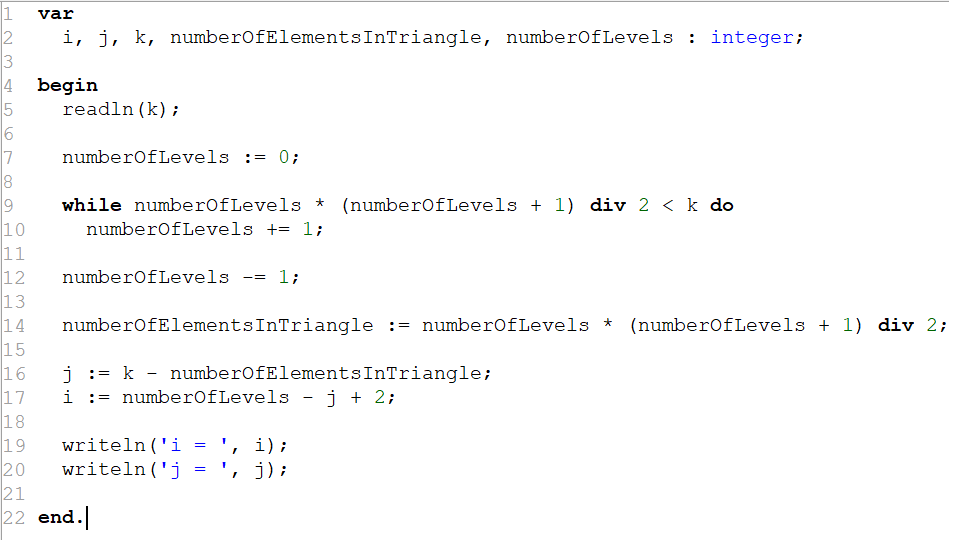
\includegraphics[scale=1.0]{task1_screenshot.png}}
	 	\caption{Решение}	 	
	 \end{figure}
 
\newpage
 
 	\textbf{Тесты:} \\[2ex]
 	
 	\begin{figure}[h]
 		\center{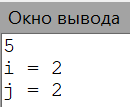
\includegraphics[scale=1.0]{task1_test1.png}}
 		\caption{Тест 1}	 	
 	\end{figure}
 
	 \begin{figure}[h]
	 	\center{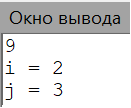
\includegraphics[scale=1.0]{task1_test2.png}}
	 	\caption{Тест 2}	 	
	 \end{figure}
 
 	\begin{figure}[h]
 		\center{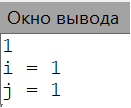
\includegraphics[scale=1.0]{task1_test3.png}}
 		\caption{Тест 3}	 	
 	\end{figure}
\end{problem}

\begin{problem}\ \\[2ex]
	Пусть $\stackrel{\wedge}{J}(w, x, y) = J(w, J(x, y))$. \\[1ex]
	Какая тройка целых $w, x, y$ приписывается числу $1000$, если \\[1ex]
	$J(x, y) = \dfrac{(x + y - 1)(x + y - 2)}{2} + y$. \\[3ex]
	
	\textbf{Решение:} \\[2ex]
	$\stackrel{\wedge}{J}(w, x, y) = J(w, J(x, y)) = 1000 := k$ \\[1ex] 
	Применим процедуру из \textbf{Задачи 1} к $k$ и найдем $J(x, y)$ и $w$. \\[1ex]
	Получим $J(x, y) = 10 := t, \ w = 36$. \\[1ex]
	Теперь применим процедуру из \textbf{Задачи 1} к $t$ и найдем $x$ и $y$. \\[1ex]
	Получим $x = 1, \ y = 4$. \\[2ex]
	
	\textbf{Ответ:} $(36, 1, 4).$ \\[4ex]
\end{problem}


\begin{problem}\ \\[1ex]
	Опишите простую процедуру для перенумерации предложений	рекурсивного язы- \\[1ex]
	ка. \\[4ex]
	
	\textbf{Решение:}
	\begin{definition}\ \\[1ex]
		Язык рекурсивен, если существует алгоритм его распознавания.
	\end{definition}

	\begin{definition}\ \\[1ex]
		Алгоритм распознавания -- алгоритм, определяющий есть ли данное предложение \\[1ex]
		в данном языке или нет.
	\end{definition}\ \\[1ex]
		$V$ -- алфавит, $L$ -- язык, $V^{*}$ -- множество всех предложений, состоящих из символов \\[1ex]
		алфавита. \\[1ex]
		Пусть в алфавите $V$ $p$ символов. Пронумеруем их числами от $0$ до $p - 1$. Поставим \\[1ex] 
		предложениям из $V^{*}$, а также предложению $\varepsilon$ в соответсвие числа из $p$-ичной \\[1ex]
		системы счисления. Реализуем это следующим образом. Предложению $\varepsilon$ \\[1ex]
		поставим в соответсвие число $0$. Пронумеруем предложения из $V^{*}$ в порядке уве- \\[1ex]
		личения длины, причём все предложения одинаковой длины будем нумеровать \\[1ex]
		в соответствии с лексикографическим порядком, определенным нумерацией \\[1ex]
		символов алфавита. \\[1ex]
		В соответствии с нумерацией будем отправлять предложения $(\varepsilon \text{ и предложения из } V^{*})$ \\[1ex]
		на проверку принадлежности языку $L$ через алгоритм распознавания. Если \\[1ex]
		предложение принадлежит языку, то ставим ему в соответсвие число $k$ \\[1ex]
		$(k = 1 \text{ изначально})$ и увеличиваем $k$ на $1$. \\[4ex]	
\end{problem}

\begin{problem}\ \\[1ex]
	Докажите, что если существует процедура для перечисления множества целых в \\[1ex] 
	монотонном порядке, то это множество рекурсивно в том смысле, что существует \\[1ex]
	алгоритм определения, находится ли данное целое в
	этом множестве. \\[2ex]
	
	\textbf{Решение:} \\[2ex]
	Хотим определить принадлежит ли число $k$ множеству. Запускаем процедуру пе- \\[1ex]
	речисления. Если текущее число, выдаваемое процедурой 
	\begin{itemize}
		\item меньше $k$, смотрим дальше;
		\item равно $k$ -- да, число $k$ принадлежит множеству, останавливаем процедуру;
		\item больше $k$ -- нет, число $k$ множеству не принадлежит, останавливаем процедуру.
	\end{itemize}
	Рассмотрим последний случай. Процедура перечисления закончила свою работу \\[1ex]
	и последнее число, которое она выдала меньше $k$. В таком случае число $k$ мно- \\[1ex]
	жеству не принадлежит. \\[1ex]
	Таким образом мы построили алгоритм определения, находится ли произвольное \\[1ex]
	целое в множестве. \\[4ex]
\end{problem}

\begin{problem}\ \\[1ex]
	Покажите, что все конечные множества рекурсивны. \\[2ex]
	
	\textbf{Решение:} \\[2ex]
	Пусть $k$ -- элемент, принадлежность множеству которого мы хотим проверить. \\[1ex]
	Множество конечно $\Rightarrow$ можно построить биекцию между элементами множества \\[1ex] 
	и целыми числами из отрезка	$[1..n]$, где $n$ -- мощность множества. В соответсвии \\[1ex] 
	с полученной нумерацией реализуем процедуру перечисления. Запустим ее. Ес- \\[1ex]
	ли текущий элемент, выдаваемый процедурой перечисления совпадает с $k$, то $k$ \\[1ex]
	принадлежит множеству, останавливаем процедуру. Если процедура завершила \\[1ex]
	свое выполнение,а про принадлежность элемента $k$ множеству не было получено \\[1ex]
	никакой информации, значит $k$ множеству не принадлежит.
\end{problem}

\end{document}